% Created 2025-07-09 Wed 12:10
% Intended LaTeX compiler: pdflatex
\documentclass[11pt]{article}
\usepackage[utf8]{inputenc}
\usepackage[T1]{fontenc}
\usepackage{graphicx}
\usepackage{longtable}
\usepackage{wrapfig}
\usepackage{rotating}
\usepackage[normalem]{ulem}
\usepackage{amsmath}
\usepackage{amssymb}
\usepackage{capt-of}
\usepackage{hyperref}
\author{Leonardo Bizzoni (899629) - Camilla Cantaluppi (894557) - Fabio Lo Presti (xxxxxx)}
\date{\today}
\title{Relazione Laboratori Coderbot}
\hypersetup{
 pdfauthor={Leonardo Bizzoni (899629) - Camilla Cantaluppi (894557) - Fabio Lo Presti (xxxxxx)},
 pdftitle={Relazione Laboratori Coderbot},
 pdfkeywords={},
 pdfsubject={},
 pdfcreator={Emacs 30.1 (Org mode 9.7.11)}, 
 pdflang={English}}
\begin{document}

\maketitle
\tableofcontents

\section{Trasformazione delle letture encoder in lunghezze degli archi percorsi}
\label{sec:org3a605c7}
L'ottenimento dei tick misurati da entrambi gli encoder, sinitro e destro, viene fatto tramite le 2 istanze di `cbEncoder\textsubscript{t}` e leggendo il valore del parametro `ticks` periodicamente:
\begin{verbatim}
cbEncoder_t cb_encoder_left = { PIN_ENCODER_LEFT_A, PIN_ENCODER_LEFT_B, -1 };
cbEncoder_t cb_encoder_right = { PIN_ENCODER_RIGHT_A, PIN_ENCODER_RIGHT_B, -1};
\end{verbatim}

I parametri di queste 2 strutture vengono aggiornati tramite due funzioni callback `cb\textsubscript{encoder}\textsubscript{callback}\textsubscript{isrA}` e `cb\textsubscript{encoder}\textsubscript{callback}\textsubscript{isrB}` che vengono invocate quando il rispettivo canale, `A` o `B`, dell'encoder invia un interrupt per segnalare il cambiamento di livello (\emph{rising o falling edge}).

\url{./img/enc-chan.gif}

La conversione del valore in tick al suo corrispondente in millimetri percorsi viene fatto grazie a 2 costanti di conversione (\emph{una per encoder}) misurante in millimetri/tick.
Queste 2 costanti sono state trovate sperimentalmente cercando di far andare il coderbot in linea retta per un albitrario intervallo di tempo e misurando la distanza percorsa con un metro e osservando quanti tick erano stati misurati dai 2 encoder. Dopo aver ripetuto l'esperimento questi sono i risultati ottenuti:
\begin{center}
\begin{tabular}{lrr}
distanza percorsa & tick encoder\textsubscript{sinistro} & tick encoder destro\\
\hline
91mm & 828 & 832\\
109mm & 965 & 970\\
98mm & 909 & 882\\
105mm & 891 & 941\\
98mm & 908 & 851\\
104mm & 925 & 938\\
\end{tabular}
\end{center}

\begin{itemize}
\item Media mm/tick encoder sinistro:            0.11147909938205335
\item Media mm/tick encoder destro:              0.1117455840579235
\item Varianza tick encoder sinistro:            1.4429498891258886e-5
\item Varianza tick encoder destro:              3.7696146281431147e-6
\item Deviazione standard tick encoder sinistro: 0.003798618023868534
\item Deviazione standard tick encoder destro:   0.0019415495430565542
\end{itemize}

Come costanti di conversione abbiamo utilizzato le 2 medie (\emph{MillimeterFromTicks\textsubscript{Left}, MillimeterFromTicks\textsubscript{Right}}).
\section{Ciclo di controllo delle ruote}
\label{sec:org781a9e5}
Il controllo delle ruote inizia leggendo il valore di velocità delle singole ruote impostato dalla task di controllo cartesiano. Questa lettura viene effettuata in sezione critica per evitare corse critiche dove la task di controllo cartesiano sovrascrive il valore di velocità mentre la task di controllo ruote cerca di leggerlo:
\begin{verbatim}
os_mutex_lock(state.speed.mutex);
// (mm/s) / (mm/tick) = (mm/s) * (tick/mm) = tick/s
f32 target_ticksXsec_left = state.speed.left / MillimeterFromTicks_Left;
f32 target_ticksXsec_right = state.speed.right / MillimeterFromTicks_Right;
os_mutex_unlock(state.speed.mutex);
\end{verbatim}
Usando un approccio a 2 task, una per ogni ruota, si potrebbe sostituire il mutex lock con un rwlock per evitare di bloccare inutilmente le 2 task di sola lettura di controllo ruote, anche se per una così breve sezione critica non porterebbe a grandi miglioramenti.

La velocità è data in millimetri al secondo ed è quindi necessario convertirla in un valore di tick che aspettiamo verranno misurati dai 2 encoder:
\begin{verbatim}
// (tick/s) * (ms / 1000ms) = tick
u64 target_ticks_left = target_ticksXsec_left * ((f32)period_ms / 1000.);
u64 target_ticks_right = target_ticksXsec_right * ((f32)period_ms / 1000.);
\end{verbatim}

Dopodiche viene determinato il nuovo duty cycle dei motori in base all'errore tra tick misurati dagli encoder e tick attesi, scalato in base alle costante proporzionali `Kp\textsubscript{Left}`, `Kp\textsubscript{Right}` e con l'aggiunta dell'errore accumulato durante l'intera esecuzione della task, scalato in base alle costanti integrali `Ki\textsubscript{Left}`, `Ki\textsubscript{Right}`.
La nuova direzione è data dal segno del duty cycle:
\begin{itemize}
\item duty cycle negativo implica che il coderbot deve muoversi indietro
\item duty cycle positivo implica che il coderbot deve muoversi in avanti
\item duty cycle nullo implica che il coderbot restare fermo e quindi la direzione è irrilevante
\end{itemize}
\begin{verbatim}
i64 delta_left = target_ticks_left - state.tick.measured_left;
i64 delta_right = target_ticks_right - state.tick.measured_right;

accumalated_error_left += delta_left;
accumalated_error_right += delta_right;

duty_cycle_left = Kp_Left * delta_left + Ki_Left * accumalated_error_left;
duty_cycle_right = Kp_Right * delta_right + Ki_Right * accumalated_error_right;

motor_direction_left = duty_cycle_left < 0 ? backward : forward;
motor_direction_right = duty_cycle_right < 0 ? backward : forward;

duty_cycle_left = Clamp(Abs(duty_cycle_left), 0.1, 0.6);
duty_cycle_right = Clamp(Abs(duty_cycle_right), 0.1, 0.6);

cb_encoder_left.ticks = 0;
cb_encoder_right.ticks = 0;
cbMotorMove(&cb_motor_left, motor_direction_left, duty_cycle_left);
cbMotorMove(&cb_motor_right, motor_direction_right, duty_cycle_right);
\end{verbatim}

Durante i test di movimento lineare del coderbot, abbiamo osservato che, con valori di duty cycle elevati, la differenza tra i tick riportati dai 2 encoder variava significativamente. I tick misurati dall'encoder sinistro erano decisamente maggiori di quelli misuarti dall'encoder destro, il che portava il robot a tendere verso la destra.
Dopo ulteriori misure abbiamo stabilito che impostare valori di duty cycle minori di `0.2` è equivalente ad un duty cycle nullo, viceversa impostando valori maggiori di `0.6`, il rapporto tra tick misurati e duty cycle non era più lineare. Per ovviare a queste 2 situazioni abbiamo quindi deciso di limitare il valore di duty cycle dei 2 encoder hai valori \(\left[0.1,0.6\right]\).
\begin{center}
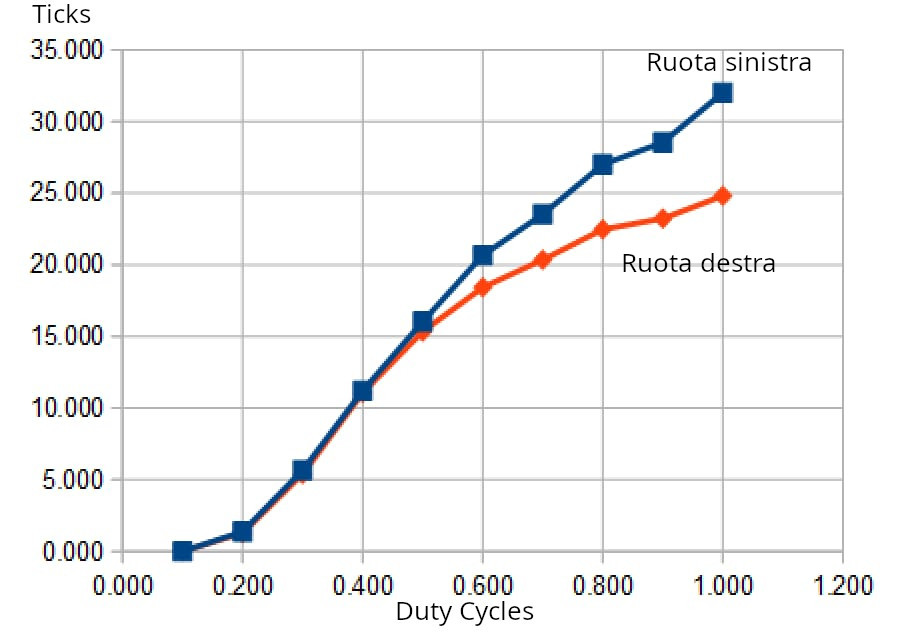
\includegraphics[width=.9\linewidth]{./img/pwm-ticks.jpg}
\end{center}

Trovare i valori delle costanti `Kp\textsubscript{Left}`, `Kp\textsubscript{Right}`, `Ki\textsubscript{Left}`, `Ki\textsubscript{Right}` è anchesso stato fatto in maniera sperimentale separatamente.
Per le costanti proporzionali si è cercato di trovarle andado a modificarle leggermente ad ogni esecuzione del programma cercando di aggiustarle per correggere l'andatura del robot. Una volta trovate queste, si è passati alle costanti integrali che, analogamente, sono state regolate gradualmente con l'obiettivo di ridurre la discrepanza tra i tick desiderati e tick misurati.
\section{Odometria}
\label{sec:org611fa9f}
\subsection{Rappresentazione delle pose del robot}
\label{sec:org3f88f4c}
\begin{center}
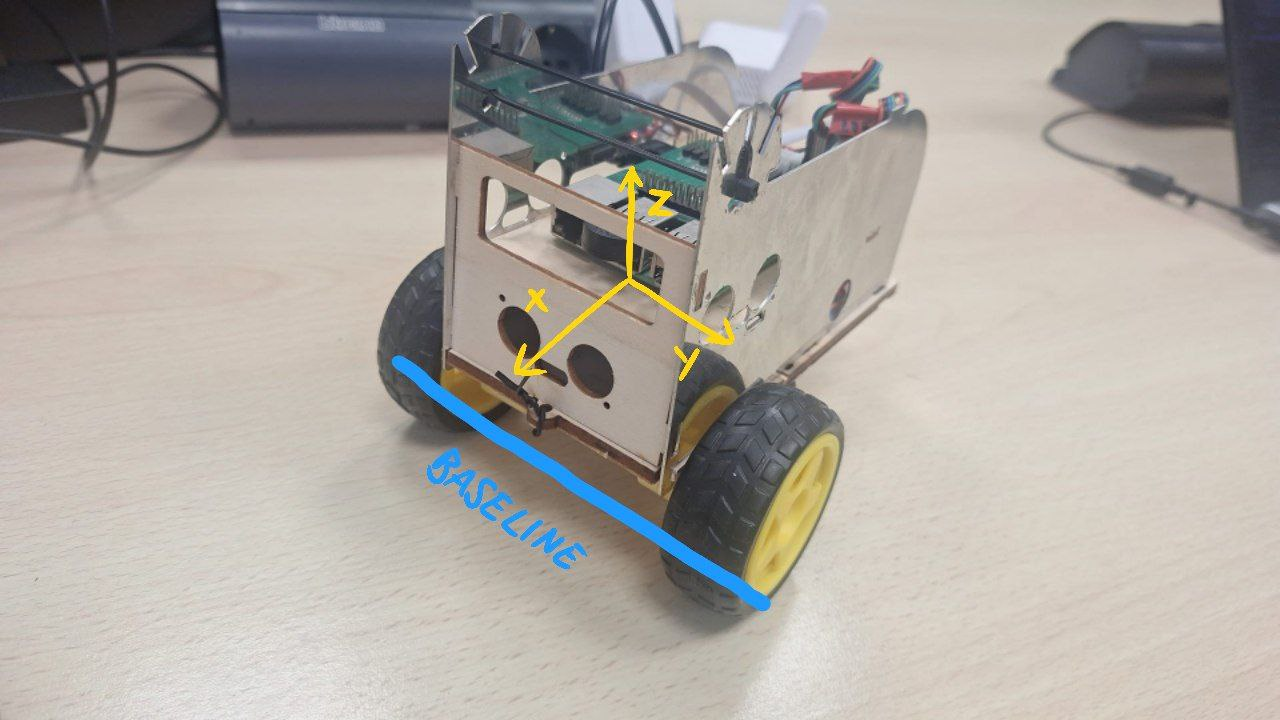
\includegraphics[width=300]{./img/coderbot-graph.jpg}
\end{center}

La pose del coderbot (\emph{la sua rotazione e posizione corrente}) viene modellata tramite una matrice \(3\times3\)  \(\text{pose}=\begin{bmatrix}R_{xx}&R_{yx}&P_x\\R_{xy}&R_{yy}&P_y\\0&0&1\end{bmatrix}\), dove:
\begin{itemize}
\item \(\bold R_{x}\) è il versore dell'asse X del sistema di riferimento attaccato al corpo del coderbot.
\item \(\bold R_{y}\) è il versore dell'asse Y del sistema di riferimento attaccato al corpo del coderbot.
\item \(\bold P\) è il vettore che indica la posizione del coderbot rispetto all'origine del sistema di riferimento attaccato al corpo del coderbot.
\end{itemize}
\subsection{Comporamente della task periodica}
\label{sec:org796a791}
Nella task di odometria vengono letti i tick misurati dagli encoder e, grazie alle costanti di conversione da tick a millimetri, si ottiene la distanza percorsa dal coderbot nel tempo percorso tra l'attivazione precedente e quella corrente della task di odometria:
\begin{verbatim}
f32 distance_left = ticks_left * MillimeterFromTicks_Left;
f32 distance_right = ticks_right * MillimeterFromTicks_Right;
\end{verbatim}

Sapendo la distanza percorsa dalle 2 ruote e la distanza tra di esse è possibile determinare l'angolo di rotazione rispetto al centro di istantanea rotazione:
\begin{verbatim}
f32 delta_theta = -(distance_left - distance_right) / BASELINE_MM;
\end{verbatim}
Per rispettare la convenzione secondo cui le rotazioni in senso antiorario hanno segno positivo, viene invertito il segno dell'angolo.
\subsubsection{Traiettoria rettilinea}
\label{sec:org0898a64}
Se l'angolo \(\theta\) è minore di una certa soglia, da noi fissata a \(0.005\text{rad}\), allora dato che la rotazione misurata è prossochè nulla, possiamo approssimare il movimento ad una linea retta lungo l'asse delle \(X\) con modulo uguale alla media delle distanze percorse dalle 2 ruote.
L'operazione da applicare alla pose attuale del coderbot sarà una semplice traslazione lungo l'asse delle X, \(\text{pose}=\text{pose}\cdot\begin{bmatrix}R&P\\0^T&1\end{bmatrix}\) dove:
\begin{itemize}
\item \(R=I_2=\begin{bmatrix}1&0\\0&1\end{bmatrix}\)
\item \(P= \begin{bmatrix}(\text{distance left} - \text{distance right})/2\\0\end{bmatrix}\)
\end{itemize}
\subsubsection{Traiettoria curviliena}
\label{sec:orgd8c175a}
Se l'angolo \(\theta\) è maggiore della soglia, questo indica che il coderbot sta effettivamente compiendo un movimento curvilineo, ruotando attorno a un centro di istantanea rotazione (\emph{CIR}). Questo CIR si trova lungo \(Y\) del sistema di riferimento del coderbot, ma traslato di una certa distanza `d`.
Il valore di `d` è dato dalla lunghezza dell'arco percorso da una delle 2 ruote, noi abbiamo deciso di considerare la ruota destra, diviso per l'angolo di rotazione. Dato che la lunghezza dell'arco è relativa alla ruota destra, è necessario sottrarre metà baseline per effettuare la traslazione rispetto al centro del coderbot:
\begin{verbatim}
f32 d = (distance_right / delta_theta) - (BASELINE_MM / 2);
\end{verbatim}

Per aggiornare la pose del coderbot, è stata applicata una rototraslazione `rt` ottenuta attraverso i seguenti passaggi:
\begin{itemize}
\item rotazione della matrice \(\text{t1}= \begin{bmatrix}1&0&0\\0&1&-d\\0&0&1\end{bmatrix}\), ovvero la matrice che esprime la posizione del CIR rispetto alla pose attuale del coderbot, di un angolo \(\theta\) rispetto l'asse Z del sistema di riferimento \emph{world}: \(R_z(\theta)\cdot\text{t1}\). Moltiplicando la pose del coderbot per questa matrice intermedia \(\text{pose}\cdot (R_z(\theta)\cdot\text{t1})\) stiamo allineando il coderbot con il CIR e vi stiamo applicando una rotazione rispetto l'asse Z.
\item applicazione di una traslazione inversa per riportare il coderbot alla posizione originale tramite moltiplicazione della matrice intermedia per \(\text{t2}= \begin{bmatrix}1&0&0\\0&1&d\\0&0&1\end{bmatrix}\), anch'essa definita nel sistema \emph{world}: \(\text{rt}=\text{t2}\cdot R_z(\theta)\cdot\text{t1}\).
\end{itemize}
Infine, la nuova pose del robot nel sistema \emph{body} è ottenuta applicando la rototraslazione `rt` alla pose corrente: \(\text{new pose} = \text{pose}\cdot\text{rt}\).
\section{Generazione della traiettoria}
\label{sec:org419c498}
Il movimento del coderbot è stabilito da un percorso predefinito, il quale viene generato offline come una sequenza di punti in un piano bidimensionale. A runtime la task di controllo cartesiano cerca il punto della traiettoria più vicino alla posizione attuale, la quale viene aggiornata dalla task di odometria, confrontando solo i punti nell'intorno della posizione corrente, al fine di determinare un obiettivo intermedio da raggiungere.

La definizione della traiettoria avviene tramite concatenzazione delle primitive di generazione di archi di rotazione e rette.
\subsection{Esempio}
\label{sec:orgfdceabc}
\begin{verbatim}
generate_arc_points(0, 900, 900, -90.f, 0.f);
generate_arc_points(1800, 900, 900, 180.f, 0.f);
generate_line_points(2700, 900, 900, -90.f);
\end{verbatim}

La prima chiamata genera un arco rispetto ad un centro di rotazione posizionato in \((0cm,90cm)\) rispetto alla posizione iniziale del coderbot e di raggio \(90cm\). I restanti 2 argomenti indicano l'angolo iniziale del robot rispetto alla circonferenza e l'angolo finale/obiettivo.

\begin{center}
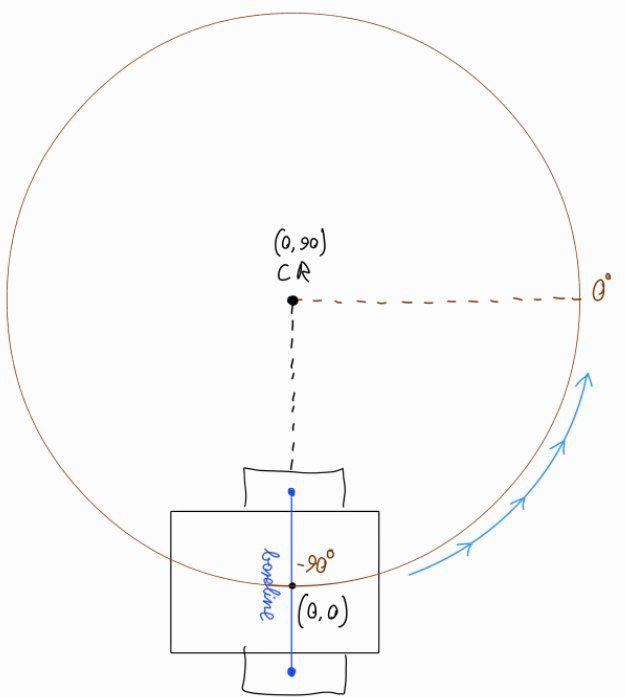
\includegraphics[width=.9\linewidth]{./img/gen_arc_example.jpg}
\end{center}

Similarmente la seconda chiamata genera un arco rispetto ad un centro di rotazione posizionato in \((180cm,90cm)\) rispetto alla posizione iniziale del coderbot e di raggio \(90cm\). La posizione di questo secondo centro di rotazione deve essere tale da potre continuare la traiettoria precedente ininterrottamente.
Infine l'ultima chiamata genera un porzione di traiettoria rettilinea con inizio alle coordinate \((270cm, 90cm)\) di lunghezza \(90cm\) e con un'inclinazione di \(-90^\circ\).

La traiettoria finale sarà:
\begin{center}
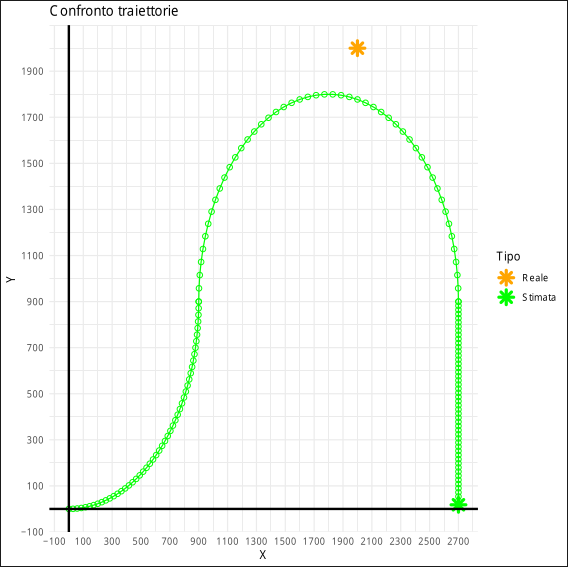
\includegraphics[width=.9\linewidth]{./img/2025-07-09-114530_hyprshot.png}
\end{center}
\end{document}
